%!TeX root=../tese.tex
%("dica" para o editor de texto: este arquivo é parte de um documento maior)
% para saber mais: https://tex.stackexchange.com/q/78101/183146

\chapter{Alguns Exemplos de Comandos \LaTeX{}}
\label{chap:exemplos}

\section{Bibliografia e Referências}

A documentação do pacote biblatex\index{biblatex} \citep{biblatex} é
bastante extensa e explica (nas Seções 2.1.1 e 2.2.2) os diversos
tipos de documento suportados, bem como o significado de cada campo.
Na prática, às vezes é preciso fazer escolhas sobre
o que incluir na descrição de um item bibliográfico e muitas vezes
é mais fácil aprender copiando exemplos já existentes, como estes (consulte o
arquivo \texttt{bibliografia.bib} para ver como foi criado o banco de dados e a
bibliografia na página \pageref{bibliografia} para ver o resultado impresso):

\begin{multicols}{2}
  \begin{itemize}
    \item @Book: \cite{Knuth:96}.

    \item @Article (em periódico): \cite{floats2014}.

    \item @InProceedings (ou @Conference): \cite{alves03:simi}.

    \item @InCollection (capítulo de livro ou coletânea): \cite{bobaoglu93:concepts}.

    \item @PhdThesis: \cite{garcia01:PhD}.

    \item @MastersThesis: \cite{schmidt03:MSc}.

    \item @Techreport: \cite{alvisi99:analysisCIC}.

    \item @Manual: \cite{biblatex}.

    \item @Misc: \cite{gridftp}.

    \item @Online (para referência a artigo \emph{online}): \cite{fowler04:designDead}.

    \item @Online (para referência a página web): \cite{FSF:GNU-GPL}.
  \end{itemize}
\end{multicols}

\section{Modo Matemático}\index{Modo Matemático}

O modo matemático do \LaTeX{} tem sintaxe própria, mas ela não é complicada e
há bastante documentação \emph{online} a respeito. Por exemplo, ``massa e
energia são grandezas relacionadas pela Equação $E=mc^2$, definida inicialmente
por Einstein'', ou ainda ``equações de segundo grau (Equação \ref{eq:2grau})
são estudadas no ensino médio. As raízes de uma equação de segundo grau podem
ser encontradas por~\eqref{eq:bhaskara} --- a fórmula de Bháskara.
O valor do discriminante $\Delta$ (Equação \ref{eq:delta}) determina se a
equação tem zero, uma ou duas raízes reais distintas''. Observe que, quando um
parágrafo termina com um símbolo, pode ser boa ideia usar um espaço
não-separável (com ``\textsf{\textasciitilde}'') para evitar que ele
fique sozinho na última linha (por exemplo, ``\textsf{O discriminante é
denotado por\textasciitilde{}\$\textbackslash{}Delta\$}'').\label{orphanchar}

\begin{equation}
  \label{eq:2grau}
  ax^2+bx+c=y \quad \forall x \in \mathbb{R}
\end{equation}

\begin{gather}
  \label{eq:bhaskara}
    y=0 \Leftrightarrow x=\frac{-b \pm \sqrt{\Delta}}{2a}
    \Leftrightarrow x \text{ é raiz da equação}\\
  \label{eq:delta}
    \Delta\enspace(\mathit{delta}) = b^2-4ac
\end{gather}

\section{\emph{Floats} (Tabelas e Figuras)}\index{Floats}

Evidentemente, \LaTeX{} permite inserir figuras no texto; além disso, ele
também permite girá-las e criar subfiguras (com sublegendas\index{Legendas}),
como no exemplo da Figura~\ref{fig:subfigures}\index{Subfiguras}, que inclui
as subfiguras \ref{fig:subfigures:a} e \ref{fig:subfigures:b}.

% As packages relevantes para lidar com figuras são graphicx,
% float, caption, rotating e subcaption. Observe que "subfigure"
% e "subtable" são definidos na package subcaption, *não* na
% package subfigure! A package subfigure é obsoleta.

%%%%%%%%% Figuras lado-a-lado %%%%%%%%%
\begin{figure}
  \centering

  \begin{subfigure}{0.4\textwidth}
    \centering
    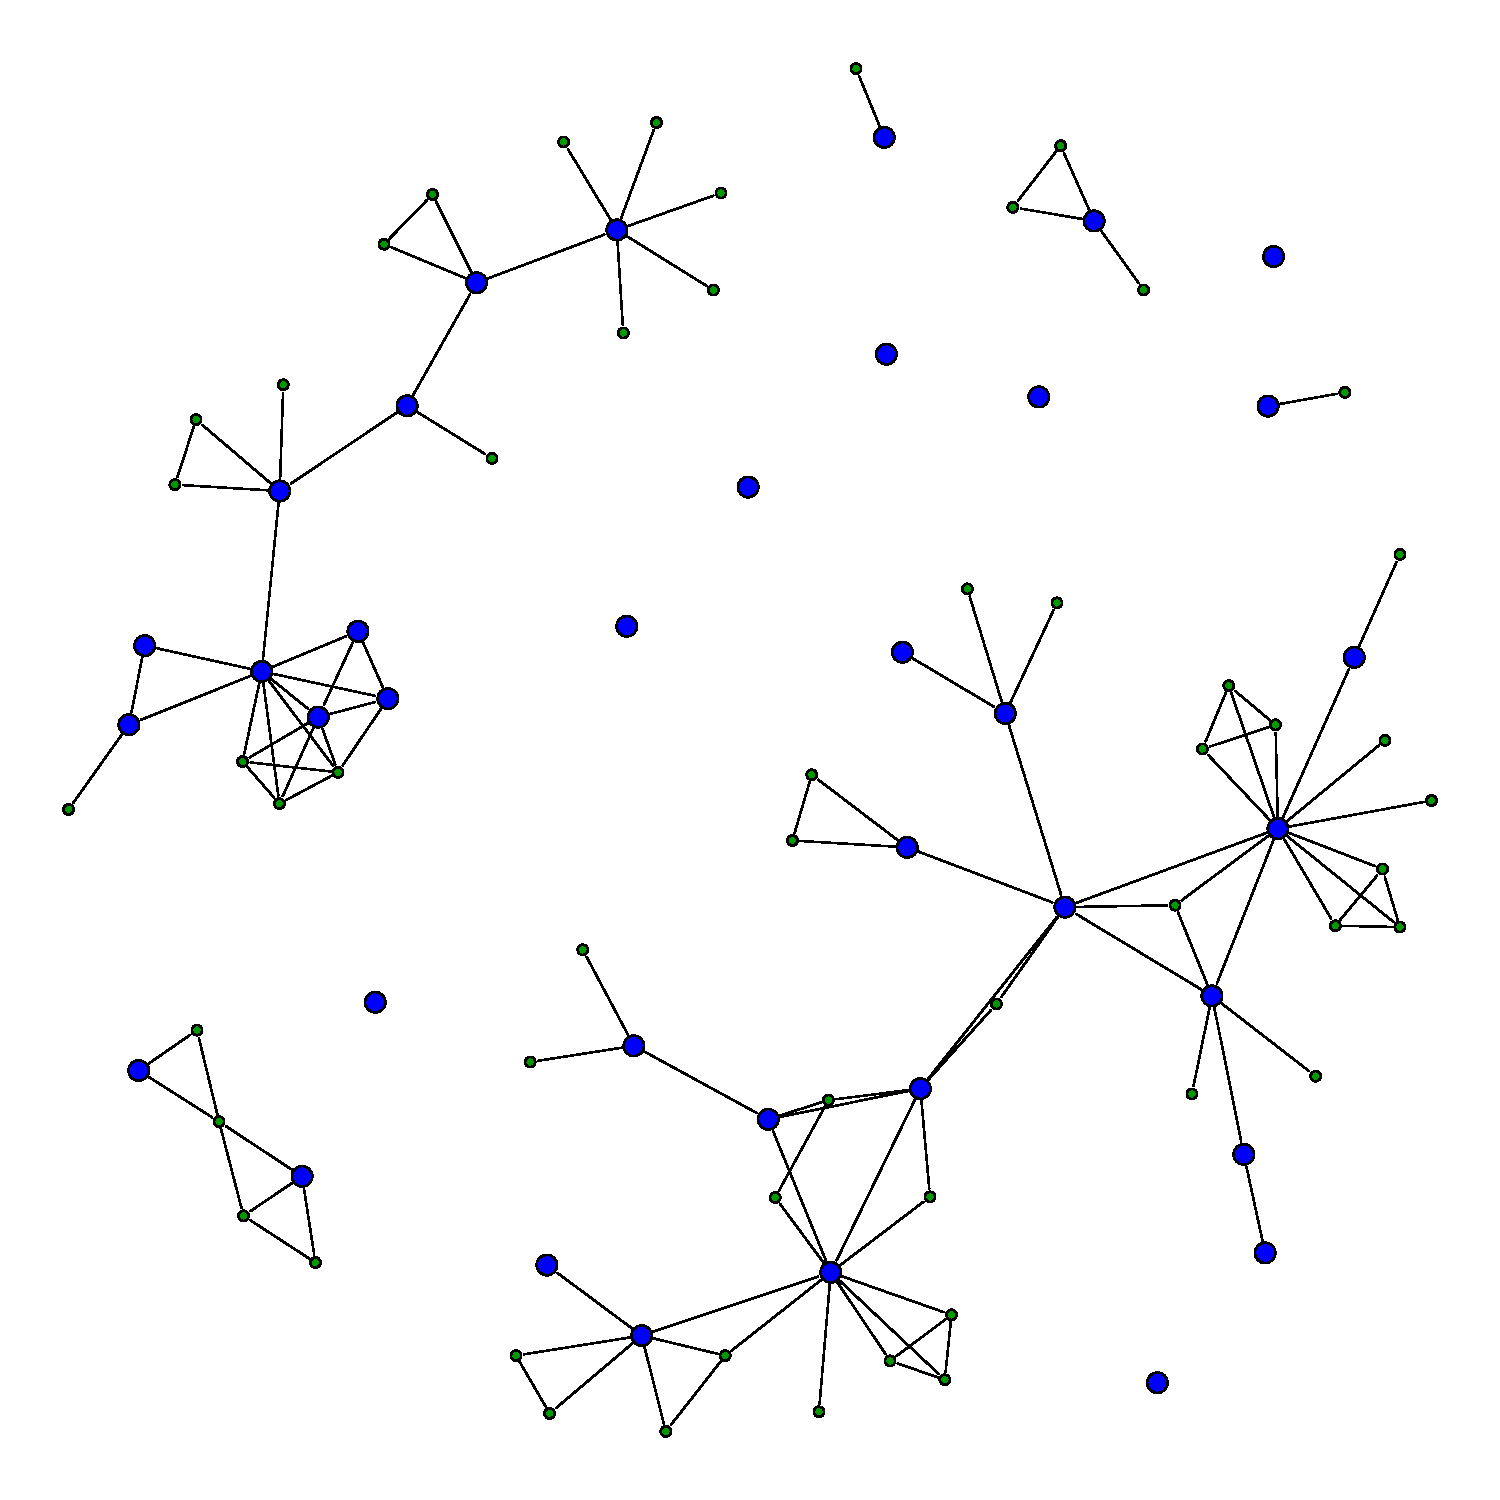
\includegraphics[width=.7\textwidth]{exemplo-grafo}
    \caption{Uma figura simples.\label{fig:subfigures:a}}
  \end{subfigure}
  % ATENÇÃO: Se você deixar uma linha em branco entre as subfiguras,
  % LaTeX vai considerar que cada uma delas pertence a um "parágrafo"
  % diferente e, portanto, vai colocá-las em linhas separadas ao invés
  % de lado a lado.
  \begin{subfigure}{0.4\textwidth}
    \centering
    \begin{turn}{90}
      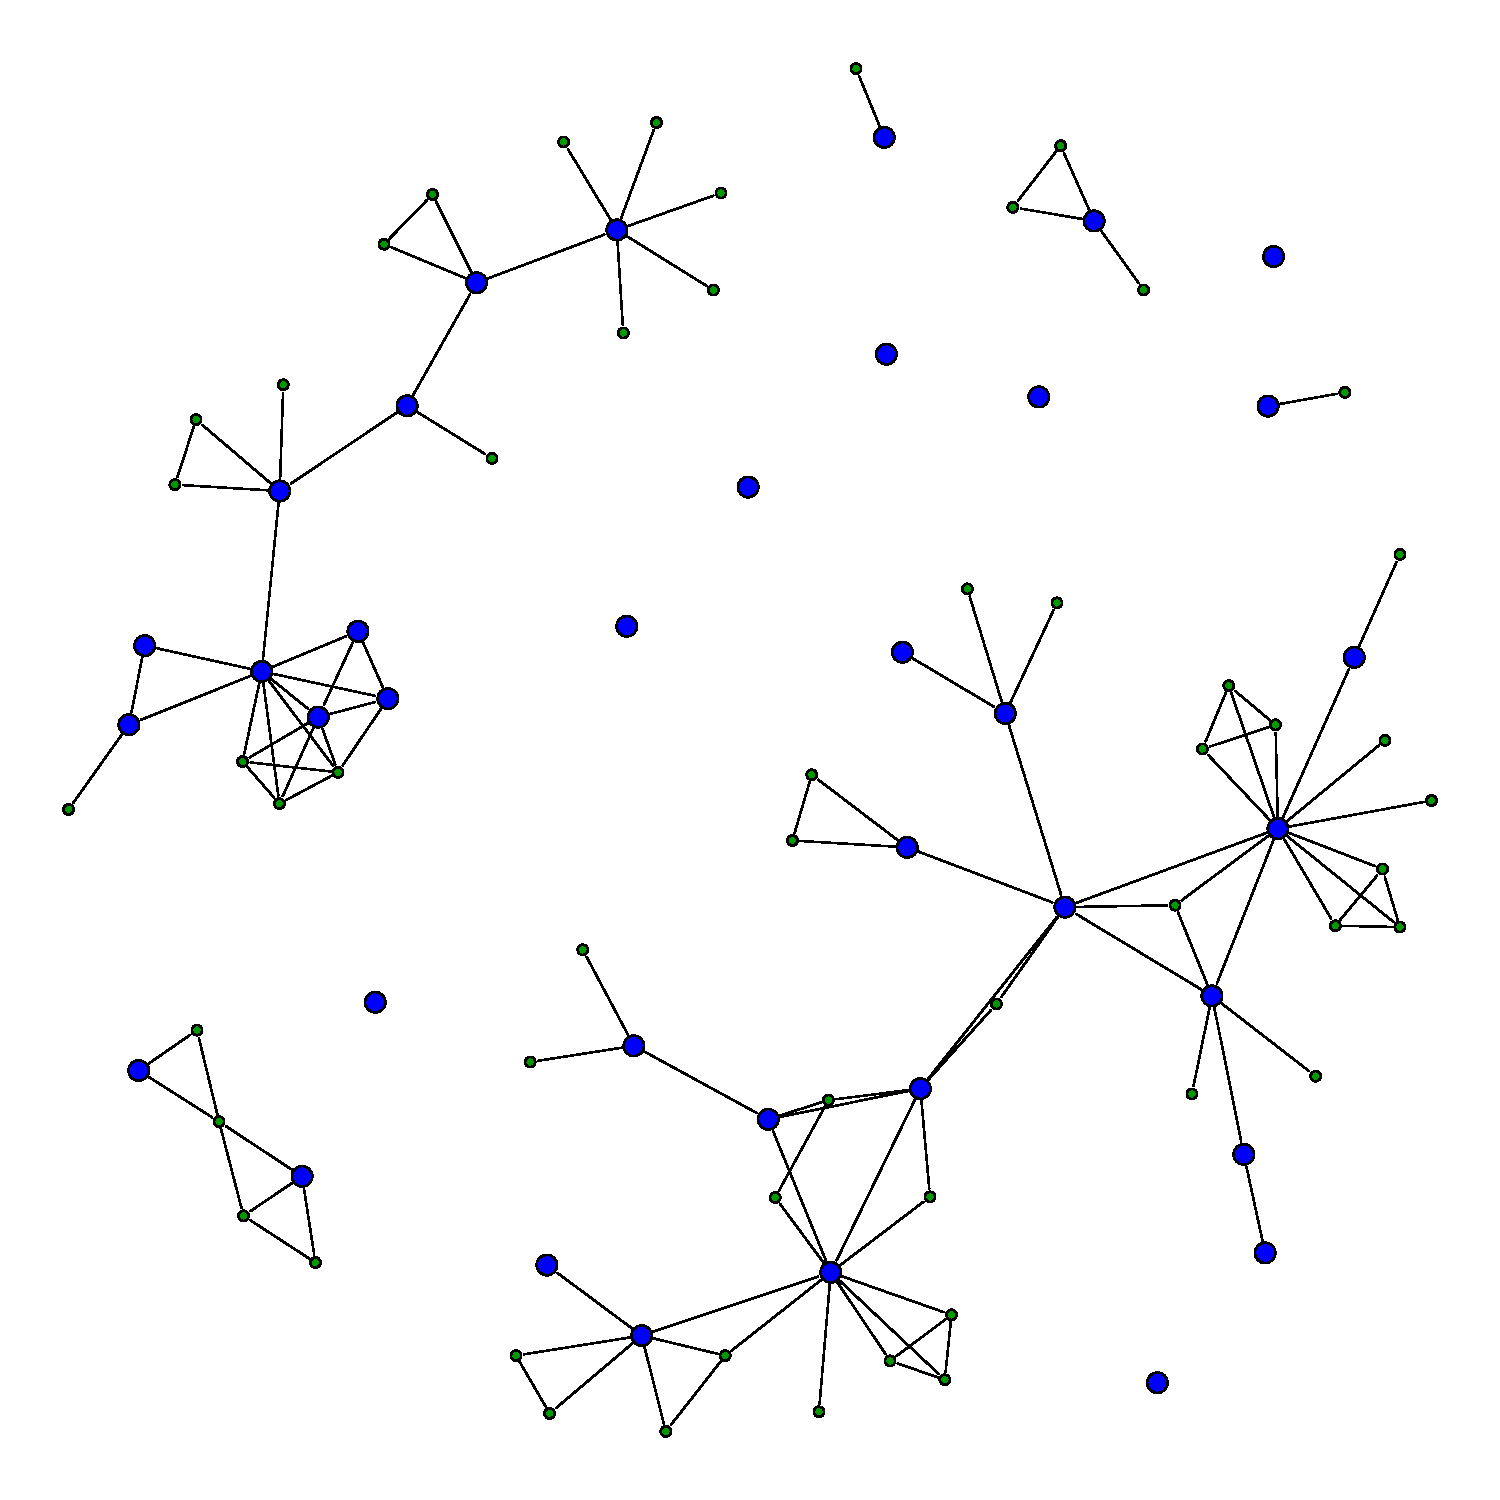
\includegraphics[width=.7\textwidth]{exemplo-grafo}
    \end{turn}
    \caption{O mesmo exemplo, girado.\label{fig:subfigures:b}}
  \end{subfigure}

  \caption{Exemplo de subfiguras.\label{fig:subfigures}}
\end{figure}

Uma ``figura'', na verdade, pode ser qualquer tipo de conteúdo ilustrativo
(um exemplo interessante é o cronograma mostrado na Figura~\ref{fig:gantt}) mas, com a
\textit{package} \textsf{float}, também é possível definir ambientes
específicos para cada tipo de conteúdo adicional (cada um com numeração
independente), como é o caso do Programa~\ref{prog:java}\index{Floats}. Há
mais informações e dicas sobre recursos específicos para inclusão de
código-fonte e pseudocódigo no Apêndice \ref{ap:pseudocode}\footnote{
Observe que o nome do Apêndice (``\ref{ap:pseudocode}'') foi impresso em
uma linha separada, o que não é muito bom visualmente. Para evitar que isso
aconteça (não só no final do parágrafo, mas em qualquer quebra de linha),
faça o que já foi discutido na Seção~\ref{orphanchar} sobre símbolos
matemáticos: utilize um espaço não-separável para fazer referências a
figuras, tabelas, seções etc.: ``\textsf{\dots no
Apêndice\textasciitilde\textbackslash{}ref\{ap:pseudocode\}}''.}.

%%%%%%% Cronograma %%%%%%%

\begin{figure}
  \centering

  % Package pgfgantt
  \begin{ganttchart}[
                     time slot format=isodate-yearmonth,
                     time slot unit=month,
                    ]{2017-11}{2018-5}

    \gantttitlecalendar{year,month=shortname} \ganttnewline

    \ganttgroup[progress=45]{Experimento}{2017-11}{2018-2} \ganttnewline
    \ganttbar[progress=100]{
      Preparação\ganttalignnewline
      (compra de insumos)
      }{2017-11}{2017-12} \ganttnewline
    \ganttbar[progress=30]{Execução}{2017-12}{2018-1} \ganttnewline
    \ganttbar[progress=0]{Análise}{2017-12}{2018-2} \ganttnewline

    \ganttgroup[progress=0]{Artigo}{2018-1}{2018-4} \ganttnewline
    \ganttbar[progress=0]{Escrita}{2018-1}{2018-3} \ganttnewline
    \ganttbar[progress=0]{Revisão}{2018-3}{2018-4} \ganttnewline

    \ganttmilestone{Submissão}{2018-4}
  \end{ganttchart}

  \caption{Exemplo de cronograma.\label{fig:gantt}}
\end{figure}

%%%%%%%% Código fonte %%%%%%%%

% Foi utilizado o pacote listings para formatar o código fonte.
% Veja os parâmetros de configuração no arquivo source-code.tex.
\begin{program}
  \index{Java}
  \centering

\begin{lstlisting}[language=Java, style=wider]
  for (i = 0; i < 20; i++)
  {
      // Comentário
      System.out.println("Mensagem...");
  }
\end{lstlisting}

  \caption{Exemplo de laço em Java.\label{prog:java}}
\end{program}

%%%%%

\LaTeX{} pode importar gráficos gerados por \texttt{matplotlib} e por
\texttt{gnuplot} como qualquer outra imagem, mas nesse caso a fonte
usada nesses gráficos provavelmente será diferente do corpo do texto.
Conforme mencionado na Seção~\ref{sec:graficos}, há mecanismos para
resolver esse problema\footnote{Você pode se interessar também pela
package \texttt{gnuplottex}.}, como pode ser visto na
Figura~\ref{fig:graficos}.

\begin{figure}
  \centering
  \begin{subfigure}{.65\textwidth}
    \input{figuras/gnuplot.tkz}
    \caption{\texttt{gnuplot}.\label{fig:gnuplot}}
  \end{subfigure}
  \begin{subfigure}{.3\textwidth}
    %% Creator: Matplotlib, PGF backend
%%
%% To include the figure in your LaTeX document, write
%%   \input{<filename>.pgf}
%%
%% Make sure the required packages are loaded in your preamble
%%   \usepackage{pgf}
%%
%% and, on pdftex
%%   \usepackage[utf8]{inputenc}\DeclareUnicodeCharacter{2212}{-}
%%
%% or, on luatex and xetex
%%   \usepackage{unicode-math}
%%
%% Figures using additional raster images can only be included by \input if
%% they are in the same directory as the main LaTeX file. For loading figures
%% from other directories you can use the `import` package
%%   \usepackage{import}
%%
%% and then include the figures with
%%   \import{<path to file>}{<filename>.pgf}
%%
%% Matplotlib used the following preamble
%%   \usepackage{fontspec}
%%   \setmainfont{DejaVuSerif.ttf}[Path=/usr/share/matplotlib/mpl-data/fonts/ttf/]
%%   \setsansfont{DejaVuSans.ttf}[Path=/usr/share/matplotlib/mpl-data/fonts/ttf/]
%%   \setmonofont{DejaVuSansMono.ttf}[Path=/usr/share/matplotlib/mpl-data/fonts/ttf/]
%%
\begingroup%
\makeatletter%
\begin{pgfpicture}%
\pgfpathrectangle{\pgfpointorigin}{\pgfqpoint{3.100000in}{1.800000in}}%
\pgfusepath{use as bounding box, clip}%
\begin{pgfscope}%
\pgfsetbuttcap%
\pgfsetmiterjoin%
\definecolor{currentfill}{rgb}{1.000000,1.000000,1.000000}%
\pgfsetfillcolor{currentfill}%
\pgfsetlinewidth{0.000000pt}%
\definecolor{currentstroke}{rgb}{1.000000,1.000000,1.000000}%
\pgfsetstrokecolor{currentstroke}%
\pgfsetdash{}{0pt}%
\pgfpathmoveto{\pgfqpoint{0.000000in}{0.000000in}}%
\pgfpathlineto{\pgfqpoint{3.100000in}{0.000000in}}%
\pgfpathlineto{\pgfqpoint{3.100000in}{1.800000in}}%
\pgfpathlineto{\pgfqpoint{0.000000in}{1.800000in}}%
\pgfpathclose%
\pgfusepath{fill}%
\end{pgfscope}%
\begin{pgfscope}%
\pgfsetbuttcap%
\pgfsetmiterjoin%
\definecolor{currentfill}{rgb}{1.000000,1.000000,1.000000}%
\pgfsetfillcolor{currentfill}%
\pgfsetlinewidth{0.000000pt}%
\definecolor{currentstroke}{rgb}{0.000000,0.000000,0.000000}%
\pgfsetstrokecolor{currentstroke}%
\pgfsetstrokeopacity{0.000000}%
\pgfsetdash{}{0pt}%
\pgfpathmoveto{\pgfqpoint{0.616528in}{0.472778in}}%
\pgfpathlineto{\pgfqpoint{2.980000in}{0.472778in}}%
\pgfpathlineto{\pgfqpoint{2.980000in}{1.680000in}}%
\pgfpathlineto{\pgfqpoint{0.616528in}{1.680000in}}%
\pgfpathclose%
\pgfusepath{fill}%
\end{pgfscope}%
\begin{pgfscope}%
\pgfsetbuttcap%
\pgfsetroundjoin%
\definecolor{currentfill}{rgb}{0.000000,0.000000,0.000000}%
\pgfsetfillcolor{currentfill}%
\pgfsetlinewidth{0.803000pt}%
\definecolor{currentstroke}{rgb}{0.000000,0.000000,0.000000}%
\pgfsetstrokecolor{currentstroke}%
\pgfsetdash{}{0pt}%
\pgfsys@defobject{currentmarker}{\pgfqpoint{0.000000in}{-0.048611in}}{\pgfqpoint{0.000000in}{0.000000in}}{%
\pgfpathmoveto{\pgfqpoint{0.000000in}{0.000000in}}%
\pgfpathlineto{\pgfqpoint{0.000000in}{-0.048611in}}%
\pgfusepath{stroke,fill}%
}%
\begin{pgfscope}%
\pgfsys@transformshift{0.822047in}{0.472778in}%
\pgfsys@useobject{currentmarker}{}%
\end{pgfscope}%
\end{pgfscope}%
\begin{pgfscope}%
\definecolor{textcolor}{rgb}{0.000000,0.000000,0.000000}%
\pgfsetstrokecolor{textcolor}%
\pgfsetfillcolor{textcolor}%
\pgftext[x=0.822047in,y=0.375556in,,top]{\color{textcolor}\sffamily\fontsize{8.000000}{9.600000}\selectfont 2}%
\end{pgfscope}%
\begin{pgfscope}%
\pgfsetbuttcap%
\pgfsetroundjoin%
\definecolor{currentfill}{rgb}{0.000000,0.000000,0.000000}%
\pgfsetfillcolor{currentfill}%
\pgfsetlinewidth{0.803000pt}%
\definecolor{currentstroke}{rgb}{0.000000,0.000000,0.000000}%
\pgfsetstrokecolor{currentstroke}%
\pgfsetdash{}{0pt}%
\pgfsys@defobject{currentmarker}{\pgfqpoint{0.000000in}{-0.048611in}}{\pgfqpoint{0.000000in}{0.000000in}}{%
\pgfpathmoveto{\pgfqpoint{0.000000in}{0.000000in}}%
\pgfpathlineto{\pgfqpoint{0.000000in}{-0.048611in}}%
\pgfusepath{stroke,fill}%
}%
\begin{pgfscope}%
\pgfsys@transformshift{1.233086in}{0.472778in}%
\pgfsys@useobject{currentmarker}{}%
\end{pgfscope}%
\end{pgfscope}%
\begin{pgfscope}%
\definecolor{textcolor}{rgb}{0.000000,0.000000,0.000000}%
\pgfsetstrokecolor{textcolor}%
\pgfsetfillcolor{textcolor}%
\pgftext[x=1.233086in,y=0.375556in,,top]{\color{textcolor}\sffamily\fontsize{8.000000}{9.600000}\selectfont 4}%
\end{pgfscope}%
\begin{pgfscope}%
\pgfsetbuttcap%
\pgfsetroundjoin%
\definecolor{currentfill}{rgb}{0.000000,0.000000,0.000000}%
\pgfsetfillcolor{currentfill}%
\pgfsetlinewidth{0.803000pt}%
\definecolor{currentstroke}{rgb}{0.000000,0.000000,0.000000}%
\pgfsetstrokecolor{currentstroke}%
\pgfsetdash{}{0pt}%
\pgfsys@defobject{currentmarker}{\pgfqpoint{0.000000in}{-0.048611in}}{\pgfqpoint{0.000000in}{0.000000in}}{%
\pgfpathmoveto{\pgfqpoint{0.000000in}{0.000000in}}%
\pgfpathlineto{\pgfqpoint{0.000000in}{-0.048611in}}%
\pgfusepath{stroke,fill}%
}%
\begin{pgfscope}%
\pgfsys@transformshift{1.644124in}{0.472778in}%
\pgfsys@useobject{currentmarker}{}%
\end{pgfscope}%
\end{pgfscope}%
\begin{pgfscope}%
\definecolor{textcolor}{rgb}{0.000000,0.000000,0.000000}%
\pgfsetstrokecolor{textcolor}%
\pgfsetfillcolor{textcolor}%
\pgftext[x=1.644124in,y=0.375556in,,top]{\color{textcolor}\sffamily\fontsize{8.000000}{9.600000}\selectfont 6}%
\end{pgfscope}%
\begin{pgfscope}%
\pgfsetbuttcap%
\pgfsetroundjoin%
\definecolor{currentfill}{rgb}{0.000000,0.000000,0.000000}%
\pgfsetfillcolor{currentfill}%
\pgfsetlinewidth{0.803000pt}%
\definecolor{currentstroke}{rgb}{0.000000,0.000000,0.000000}%
\pgfsetstrokecolor{currentstroke}%
\pgfsetdash{}{0pt}%
\pgfsys@defobject{currentmarker}{\pgfqpoint{0.000000in}{-0.048611in}}{\pgfqpoint{0.000000in}{0.000000in}}{%
\pgfpathmoveto{\pgfqpoint{0.000000in}{0.000000in}}%
\pgfpathlineto{\pgfqpoint{0.000000in}{-0.048611in}}%
\pgfusepath{stroke,fill}%
}%
\begin{pgfscope}%
\pgfsys@transformshift{2.055163in}{0.472778in}%
\pgfsys@useobject{currentmarker}{}%
\end{pgfscope}%
\end{pgfscope}%
\begin{pgfscope}%
\definecolor{textcolor}{rgb}{0.000000,0.000000,0.000000}%
\pgfsetstrokecolor{textcolor}%
\pgfsetfillcolor{textcolor}%
\pgftext[x=2.055163in,y=0.375556in,,top]{\color{textcolor}\sffamily\fontsize{8.000000}{9.600000}\selectfont 8}%
\end{pgfscope}%
\begin{pgfscope}%
\pgfsetbuttcap%
\pgfsetroundjoin%
\definecolor{currentfill}{rgb}{0.000000,0.000000,0.000000}%
\pgfsetfillcolor{currentfill}%
\pgfsetlinewidth{0.803000pt}%
\definecolor{currentstroke}{rgb}{0.000000,0.000000,0.000000}%
\pgfsetstrokecolor{currentstroke}%
\pgfsetdash{}{0pt}%
\pgfsys@defobject{currentmarker}{\pgfqpoint{0.000000in}{-0.048611in}}{\pgfqpoint{0.000000in}{0.000000in}}{%
\pgfpathmoveto{\pgfqpoint{0.000000in}{0.000000in}}%
\pgfpathlineto{\pgfqpoint{0.000000in}{-0.048611in}}%
\pgfusepath{stroke,fill}%
}%
\begin{pgfscope}%
\pgfsys@transformshift{2.466202in}{0.472778in}%
\pgfsys@useobject{currentmarker}{}%
\end{pgfscope}%
\end{pgfscope}%
\begin{pgfscope}%
\definecolor{textcolor}{rgb}{0.000000,0.000000,0.000000}%
\pgfsetstrokecolor{textcolor}%
\pgfsetfillcolor{textcolor}%
\pgftext[x=2.466202in,y=0.375556in,,top]{\color{textcolor}\sffamily\fontsize{8.000000}{9.600000}\selectfont 10}%
\end{pgfscope}%
\begin{pgfscope}%
\pgfsetbuttcap%
\pgfsetroundjoin%
\definecolor{currentfill}{rgb}{0.000000,0.000000,0.000000}%
\pgfsetfillcolor{currentfill}%
\pgfsetlinewidth{0.803000pt}%
\definecolor{currentstroke}{rgb}{0.000000,0.000000,0.000000}%
\pgfsetstrokecolor{currentstroke}%
\pgfsetdash{}{0pt}%
\pgfsys@defobject{currentmarker}{\pgfqpoint{0.000000in}{-0.048611in}}{\pgfqpoint{0.000000in}{0.000000in}}{%
\pgfpathmoveto{\pgfqpoint{0.000000in}{0.000000in}}%
\pgfpathlineto{\pgfqpoint{0.000000in}{-0.048611in}}%
\pgfusepath{stroke,fill}%
}%
\begin{pgfscope}%
\pgfsys@transformshift{2.877240in}{0.472778in}%
\pgfsys@useobject{currentmarker}{}%
\end{pgfscope}%
\end{pgfscope}%
\begin{pgfscope}%
\definecolor{textcolor}{rgb}{0.000000,0.000000,0.000000}%
\pgfsetstrokecolor{textcolor}%
\pgfsetfillcolor{textcolor}%
\pgftext[x=2.877240in,y=0.375556in,,top]{\color{textcolor}\sffamily\fontsize{8.000000}{9.600000}\selectfont 12}%
\end{pgfscope}%
\begin{pgfscope}%
\definecolor{textcolor}{rgb}{0.000000,0.000000,0.000000}%
\pgfsetstrokecolor{textcolor}%
\pgfsetfillcolor{textcolor}%
\pgftext[x=1.798264in,y=0.212470in,,top]{\color{textcolor}\sffamily\fontsize{8.000000}{9.600000}\selectfont \(\displaystyle x\)}%
\end{pgfscope}%
\begin{pgfscope}%
\pgfsetbuttcap%
\pgfsetroundjoin%
\definecolor{currentfill}{rgb}{0.000000,0.000000,0.000000}%
\pgfsetfillcolor{currentfill}%
\pgfsetlinewidth{0.803000pt}%
\definecolor{currentstroke}{rgb}{0.000000,0.000000,0.000000}%
\pgfsetstrokecolor{currentstroke}%
\pgfsetdash{}{0pt}%
\pgfsys@defobject{currentmarker}{\pgfqpoint{-0.048611in}{0.000000in}}{\pgfqpoint{-0.000000in}{0.000000in}}{%
\pgfpathmoveto{\pgfqpoint{-0.000000in}{0.000000in}}%
\pgfpathlineto{\pgfqpoint{-0.048611in}{0.000000in}}%
\pgfusepath{stroke,fill}%
}%
\begin{pgfscope}%
\pgfsys@transformshift{0.616528in}{0.472778in}%
\pgfsys@useobject{currentmarker}{}%
\end{pgfscope}%
\end{pgfscope}%
\begin{pgfscope}%
\definecolor{textcolor}{rgb}{0.000000,0.000000,0.000000}%
\pgfsetstrokecolor{textcolor}%
\pgfsetfillcolor{textcolor}%
\pgftext[x=0.448613in, y=0.430569in, left, base]{\color{textcolor}\sffamily\fontsize{8.000000}{9.600000}\selectfont 0}%
\end{pgfscope}%
\begin{pgfscope}%
\pgfsetbuttcap%
\pgfsetroundjoin%
\definecolor{currentfill}{rgb}{0.000000,0.000000,0.000000}%
\pgfsetfillcolor{currentfill}%
\pgfsetlinewidth{0.803000pt}%
\definecolor{currentstroke}{rgb}{0.000000,0.000000,0.000000}%
\pgfsetstrokecolor{currentstroke}%
\pgfsetdash{}{0pt}%
\pgfsys@defobject{currentmarker}{\pgfqpoint{-0.048611in}{0.000000in}}{\pgfqpoint{-0.000000in}{0.000000in}}{%
\pgfpathmoveto{\pgfqpoint{-0.000000in}{0.000000in}}%
\pgfpathlineto{\pgfqpoint{-0.048611in}{0.000000in}}%
\pgfusepath{stroke,fill}%
}%
\begin{pgfscope}%
\pgfsys@transformshift{0.616528in}{0.680920in}%
\pgfsys@useobject{currentmarker}{}%
\end{pgfscope}%
\end{pgfscope}%
\begin{pgfscope}%
\definecolor{textcolor}{rgb}{0.000000,0.000000,0.000000}%
\pgfsetstrokecolor{textcolor}%
\pgfsetfillcolor{textcolor}%
\pgftext[x=0.377921in, y=0.638710in, left, base]{\color{textcolor}\sffamily\fontsize{8.000000}{9.600000}\selectfont 25}%
\end{pgfscope}%
\begin{pgfscope}%
\pgfsetbuttcap%
\pgfsetroundjoin%
\definecolor{currentfill}{rgb}{0.000000,0.000000,0.000000}%
\pgfsetfillcolor{currentfill}%
\pgfsetlinewidth{0.803000pt}%
\definecolor{currentstroke}{rgb}{0.000000,0.000000,0.000000}%
\pgfsetstrokecolor{currentstroke}%
\pgfsetdash{}{0pt}%
\pgfsys@defobject{currentmarker}{\pgfqpoint{-0.048611in}{0.000000in}}{\pgfqpoint{-0.000000in}{0.000000in}}{%
\pgfpathmoveto{\pgfqpoint{-0.000000in}{0.000000in}}%
\pgfpathlineto{\pgfqpoint{-0.048611in}{0.000000in}}%
\pgfusepath{stroke,fill}%
}%
\begin{pgfscope}%
\pgfsys@transformshift{0.616528in}{0.889061in}%
\pgfsys@useobject{currentmarker}{}%
\end{pgfscope}%
\end{pgfscope}%
\begin{pgfscope}%
\definecolor{textcolor}{rgb}{0.000000,0.000000,0.000000}%
\pgfsetstrokecolor{textcolor}%
\pgfsetfillcolor{textcolor}%
\pgftext[x=0.377921in, y=0.846852in, left, base]{\color{textcolor}\sffamily\fontsize{8.000000}{9.600000}\selectfont 50}%
\end{pgfscope}%
\begin{pgfscope}%
\pgfsetbuttcap%
\pgfsetroundjoin%
\definecolor{currentfill}{rgb}{0.000000,0.000000,0.000000}%
\pgfsetfillcolor{currentfill}%
\pgfsetlinewidth{0.803000pt}%
\definecolor{currentstroke}{rgb}{0.000000,0.000000,0.000000}%
\pgfsetstrokecolor{currentstroke}%
\pgfsetdash{}{0pt}%
\pgfsys@defobject{currentmarker}{\pgfqpoint{-0.048611in}{0.000000in}}{\pgfqpoint{-0.000000in}{0.000000in}}{%
\pgfpathmoveto{\pgfqpoint{-0.000000in}{0.000000in}}%
\pgfpathlineto{\pgfqpoint{-0.048611in}{0.000000in}}%
\pgfusepath{stroke,fill}%
}%
\begin{pgfscope}%
\pgfsys@transformshift{0.616528in}{1.097203in}%
\pgfsys@useobject{currentmarker}{}%
\end{pgfscope}%
\end{pgfscope}%
\begin{pgfscope}%
\definecolor{textcolor}{rgb}{0.000000,0.000000,0.000000}%
\pgfsetstrokecolor{textcolor}%
\pgfsetfillcolor{textcolor}%
\pgftext[x=0.377921in, y=1.054994in, left, base]{\color{textcolor}\sffamily\fontsize{8.000000}{9.600000}\selectfont 75}%
\end{pgfscope}%
\begin{pgfscope}%
\pgfsetbuttcap%
\pgfsetroundjoin%
\definecolor{currentfill}{rgb}{0.000000,0.000000,0.000000}%
\pgfsetfillcolor{currentfill}%
\pgfsetlinewidth{0.803000pt}%
\definecolor{currentstroke}{rgb}{0.000000,0.000000,0.000000}%
\pgfsetstrokecolor{currentstroke}%
\pgfsetdash{}{0pt}%
\pgfsys@defobject{currentmarker}{\pgfqpoint{-0.048611in}{0.000000in}}{\pgfqpoint{-0.000000in}{0.000000in}}{%
\pgfpathmoveto{\pgfqpoint{-0.000000in}{0.000000in}}%
\pgfpathlineto{\pgfqpoint{-0.048611in}{0.000000in}}%
\pgfusepath{stroke,fill}%
}%
\begin{pgfscope}%
\pgfsys@transformshift{0.616528in}{1.305345in}%
\pgfsys@useobject{currentmarker}{}%
\end{pgfscope}%
\end{pgfscope}%
\begin{pgfscope}%
\definecolor{textcolor}{rgb}{0.000000,0.000000,0.000000}%
\pgfsetstrokecolor{textcolor}%
\pgfsetfillcolor{textcolor}%
\pgftext[x=0.307229in, y=1.263136in, left, base]{\color{textcolor}\sffamily\fontsize{8.000000}{9.600000}\selectfont 100}%
\end{pgfscope}%
\begin{pgfscope}%
\pgfsetbuttcap%
\pgfsetroundjoin%
\definecolor{currentfill}{rgb}{0.000000,0.000000,0.000000}%
\pgfsetfillcolor{currentfill}%
\pgfsetlinewidth{0.803000pt}%
\definecolor{currentstroke}{rgb}{0.000000,0.000000,0.000000}%
\pgfsetstrokecolor{currentstroke}%
\pgfsetdash{}{0pt}%
\pgfsys@defobject{currentmarker}{\pgfqpoint{-0.048611in}{0.000000in}}{\pgfqpoint{-0.000000in}{0.000000in}}{%
\pgfpathmoveto{\pgfqpoint{-0.000000in}{0.000000in}}%
\pgfpathlineto{\pgfqpoint{-0.048611in}{0.000000in}}%
\pgfusepath{stroke,fill}%
}%
\begin{pgfscope}%
\pgfsys@transformshift{0.616528in}{1.513487in}%
\pgfsys@useobject{currentmarker}{}%
\end{pgfscope}%
\end{pgfscope}%
\begin{pgfscope}%
\definecolor{textcolor}{rgb}{0.000000,0.000000,0.000000}%
\pgfsetstrokecolor{textcolor}%
\pgfsetfillcolor{textcolor}%
\pgftext[x=0.307229in, y=1.471277in, left, base]{\color{textcolor}\sffamily\fontsize{8.000000}{9.600000}\selectfont 125}%
\end{pgfscope}%
\begin{pgfscope}%
\definecolor{textcolor}{rgb}{0.000000,0.000000,0.000000}%
\pgfsetstrokecolor{textcolor}%
\pgfsetfillcolor{textcolor}%
\pgftext[x=0.251673in,y=1.076389in,,bottom,rotate=90.000000]{\color{textcolor}\sffamily\fontsize{8.000000}{9.600000}\selectfont \(\displaystyle f(x)\)}%
\end{pgfscope}%
\begin{pgfscope}%
\pgfpathrectangle{\pgfqpoint{0.616528in}{0.472778in}}{\pgfqpoint{2.363472in}{1.207222in}}%
\pgfusepath{clip}%
\pgfsetbuttcap%
\pgfsetroundjoin%
\pgfsetlinewidth{0.501875pt}%
\definecolor{currentstroke}{rgb}{0.172549,0.627451,0.172549}%
\pgfsetstrokecolor{currentstroke}%
\pgfsetdash{}{0pt}%
\pgfpathmoveto{\pgfqpoint{0.616528in}{0.472778in}}%
\pgfpathlineto{\pgfqpoint{0.616528in}{0.472778in}}%
\pgfusepath{stroke}%
\end{pgfscope}%
\begin{pgfscope}%
\pgfpathrectangle{\pgfqpoint{0.616528in}{0.472778in}}{\pgfqpoint{2.363472in}{1.207222in}}%
\pgfusepath{clip}%
\pgfsetbuttcap%
\pgfsetroundjoin%
\pgfsetlinewidth{0.501875pt}%
\definecolor{currentstroke}{rgb}{0.172549,0.627451,0.172549}%
\pgfsetstrokecolor{currentstroke}%
\pgfsetdash{}{0pt}%
\pgfpathmoveto{\pgfqpoint{0.719287in}{0.568690in}}%
\pgfpathlineto{\pgfqpoint{0.719287in}{0.651114in}}%
\pgfusepath{stroke}%
\end{pgfscope}%
\begin{pgfscope}%
\pgfpathrectangle{\pgfqpoint{0.616528in}{0.472778in}}{\pgfqpoint{2.363472in}{1.207222in}}%
\pgfusepath{clip}%
\pgfsetbuttcap%
\pgfsetroundjoin%
\pgfsetlinewidth{0.501875pt}%
\definecolor{currentstroke}{rgb}{0.172549,0.627451,0.172549}%
\pgfsetstrokecolor{currentstroke}%
\pgfsetdash{}{0pt}%
\pgfpathmoveto{\pgfqpoint{0.822047in}{0.636793in}}%
\pgfpathlineto{\pgfqpoint{0.822047in}{0.712557in}}%
\pgfusepath{stroke}%
\end{pgfscope}%
\begin{pgfscope}%
\pgfpathrectangle{\pgfqpoint{0.616528in}{0.472778in}}{\pgfqpoint{2.363472in}{1.207222in}}%
\pgfusepath{clip}%
\pgfsetbuttcap%
\pgfsetroundjoin%
\pgfsetlinewidth{0.501875pt}%
\definecolor{currentstroke}{rgb}{0.172549,0.627451,0.172549}%
\pgfsetstrokecolor{currentstroke}%
\pgfsetdash{}{0pt}%
\pgfpathmoveto{\pgfqpoint{1.027566in}{0.771836in}}%
\pgfpathlineto{\pgfqpoint{1.027566in}{0.854260in}}%
\pgfusepath{stroke}%
\end{pgfscope}%
\begin{pgfscope}%
\pgfpathrectangle{\pgfqpoint{0.616528in}{0.472778in}}{\pgfqpoint{2.363472in}{1.207222in}}%
\pgfusepath{clip}%
\pgfsetbuttcap%
\pgfsetroundjoin%
\pgfsetlinewidth{0.501875pt}%
\definecolor{currentstroke}{rgb}{0.172549,0.627451,0.172549}%
\pgfsetstrokecolor{currentstroke}%
\pgfsetdash{}{0pt}%
\pgfpathmoveto{\pgfqpoint{1.438605in}{0.937766in}}%
\pgfpathlineto{\pgfqpoint{1.438605in}{1.001874in}}%
\pgfusepath{stroke}%
\end{pgfscope}%
\begin{pgfscope}%
\pgfpathrectangle{\pgfqpoint{0.616528in}{0.472778in}}{\pgfqpoint{2.363472in}{1.207222in}}%
\pgfusepath{clip}%
\pgfsetbuttcap%
\pgfsetroundjoin%
\pgfsetlinewidth{0.501875pt}%
\definecolor{currentstroke}{rgb}{0.172549,0.627451,0.172549}%
\pgfsetstrokecolor{currentstroke}%
\pgfsetdash{}{0pt}%
\pgfpathmoveto{\pgfqpoint{1.849644in}{1.024603in}}%
\pgfpathlineto{\pgfqpoint{1.849644in}{1.112023in}}%
\pgfusepath{stroke}%
\end{pgfscope}%
\begin{pgfscope}%
\pgfpathrectangle{\pgfqpoint{0.616528in}{0.472778in}}{\pgfqpoint{2.363472in}{1.207222in}}%
\pgfusepath{clip}%
\pgfsetbuttcap%
\pgfsetroundjoin%
\pgfsetlinewidth{0.501875pt}%
\definecolor{currentstroke}{rgb}{0.172549,0.627451,0.172549}%
\pgfsetstrokecolor{currentstroke}%
\pgfsetdash{}{0pt}%
\pgfpathmoveto{\pgfqpoint{2.055163in}{1.031430in}}%
\pgfpathlineto{\pgfqpoint{2.055163in}{1.116352in}}%
\pgfusepath{stroke}%
\end{pgfscope}%
\begin{pgfscope}%
\pgfpathrectangle{\pgfqpoint{0.616528in}{0.472778in}}{\pgfqpoint{2.363472in}{1.207222in}}%
\pgfusepath{clip}%
\pgfsetbuttcap%
\pgfsetroundjoin%
\pgfsetlinewidth{0.501875pt}%
\definecolor{currentstroke}{rgb}{0.172549,0.627451,0.172549}%
\pgfsetstrokecolor{currentstroke}%
\pgfsetdash{}{0pt}%
\pgfpathmoveto{\pgfqpoint{2.856688in}{1.150654in}}%
\pgfpathlineto{\pgfqpoint{2.856688in}{1.248064in}}%
\pgfusepath{stroke}%
\end{pgfscope}%
\begin{pgfscope}%
\pgfpathrectangle{\pgfqpoint{0.616528in}{0.472778in}}{\pgfqpoint{2.363472in}{1.207222in}}%
\pgfusepath{clip}%
\pgfsetrectcap%
\pgfsetroundjoin%
\pgfsetlinewidth{1.003750pt}%
\definecolor{currentstroke}{rgb}{0.121569,0.466667,0.705882}%
\pgfsetstrokecolor{currentstroke}%
\pgfsetdash{}{0pt}%
\pgfpathmoveto{\pgfqpoint{0.616528in}{0.472778in}}%
\pgfpathlineto{\pgfqpoint{0.637080in}{0.481103in}}%
\pgfpathlineto{\pgfqpoint{0.657632in}{0.489429in}}%
\pgfpathlineto{\pgfqpoint{0.678184in}{0.497755in}}%
\pgfpathlineto{\pgfqpoint{0.698736in}{0.506080in}}%
\pgfpathlineto{\pgfqpoint{0.719287in}{0.514406in}}%
\pgfpathlineto{\pgfqpoint{0.739839in}{0.522732in}}%
\pgfpathlineto{\pgfqpoint{0.760391in}{0.531057in}}%
\pgfpathlineto{\pgfqpoint{0.780943in}{0.539383in}}%
\pgfpathlineto{\pgfqpoint{0.801495in}{0.547709in}}%
\pgfpathlineto{\pgfqpoint{0.822047in}{0.556034in}}%
\pgfpathlineto{\pgfqpoint{0.842599in}{0.564360in}}%
\pgfpathlineto{\pgfqpoint{0.863151in}{0.572686in}}%
\pgfpathlineto{\pgfqpoint{0.883703in}{0.581011in}}%
\pgfpathlineto{\pgfqpoint{0.904255in}{0.589337in}}%
\pgfpathlineto{\pgfqpoint{0.924807in}{0.597663in}}%
\pgfpathlineto{\pgfqpoint{0.945359in}{0.605989in}}%
\pgfpathlineto{\pgfqpoint{0.965911in}{0.614314in}}%
\pgfpathlineto{\pgfqpoint{0.986463in}{0.622640in}}%
\pgfpathlineto{\pgfqpoint{1.007014in}{0.630966in}}%
\pgfpathlineto{\pgfqpoint{1.027566in}{0.639291in}}%
\pgfpathlineto{\pgfqpoint{1.048118in}{0.647617in}}%
\pgfpathlineto{\pgfqpoint{1.068670in}{0.655943in}}%
\pgfpathlineto{\pgfqpoint{1.089222in}{0.664268in}}%
\pgfpathlineto{\pgfqpoint{1.109774in}{0.672594in}}%
\pgfpathlineto{\pgfqpoint{1.130326in}{0.680920in}}%
\pgfpathlineto{\pgfqpoint{1.150878in}{0.689245in}}%
\pgfpathlineto{\pgfqpoint{1.171430in}{0.697571in}}%
\pgfpathlineto{\pgfqpoint{1.191982in}{0.705897in}}%
\pgfpathlineto{\pgfqpoint{1.212534in}{0.714222in}}%
\pgfpathlineto{\pgfqpoint{1.233086in}{0.722548in}}%
\pgfpathlineto{\pgfqpoint{1.253638in}{0.730874in}}%
\pgfpathlineto{\pgfqpoint{1.274190in}{0.739199in}}%
\pgfpathlineto{\pgfqpoint{1.294742in}{0.747525in}}%
\pgfpathlineto{\pgfqpoint{1.315293in}{0.755851in}}%
\pgfpathlineto{\pgfqpoint{1.335845in}{0.764176in}}%
\pgfpathlineto{\pgfqpoint{1.356397in}{0.772502in}}%
\pgfpathlineto{\pgfqpoint{1.376949in}{0.780828in}}%
\pgfpathlineto{\pgfqpoint{1.397501in}{0.789153in}}%
\pgfpathlineto{\pgfqpoint{1.418053in}{0.797479in}}%
\pgfpathlineto{\pgfqpoint{1.438605in}{0.805805in}}%
\pgfpathlineto{\pgfqpoint{1.459157in}{0.814130in}}%
\pgfpathlineto{\pgfqpoint{1.479709in}{0.822456in}}%
\pgfpathlineto{\pgfqpoint{1.500261in}{0.830782in}}%
\pgfpathlineto{\pgfqpoint{1.520813in}{0.839107in}}%
\pgfpathlineto{\pgfqpoint{1.541365in}{0.847433in}}%
\pgfpathlineto{\pgfqpoint{1.561917in}{0.855759in}}%
\pgfpathlineto{\pgfqpoint{1.582469in}{0.864084in}}%
\pgfpathlineto{\pgfqpoint{1.603021in}{0.872410in}}%
\pgfpathlineto{\pgfqpoint{1.623572in}{0.880736in}}%
\pgfpathlineto{\pgfqpoint{1.644124in}{0.889061in}}%
\pgfpathlineto{\pgfqpoint{1.664676in}{0.897387in}}%
\pgfpathlineto{\pgfqpoint{1.685228in}{0.905713in}}%
\pgfpathlineto{\pgfqpoint{1.705780in}{0.914038in}}%
\pgfpathlineto{\pgfqpoint{1.726332in}{0.922364in}}%
\pgfpathlineto{\pgfqpoint{1.746884in}{0.930690in}}%
\pgfpathlineto{\pgfqpoint{1.767436in}{0.939015in}}%
\pgfpathlineto{\pgfqpoint{1.787988in}{0.947341in}}%
\pgfpathlineto{\pgfqpoint{1.808540in}{0.955667in}}%
\pgfpathlineto{\pgfqpoint{1.829092in}{0.963992in}}%
\pgfpathlineto{\pgfqpoint{1.849644in}{0.972318in}}%
\pgfpathlineto{\pgfqpoint{1.870196in}{0.980644in}}%
\pgfpathlineto{\pgfqpoint{1.890748in}{0.988969in}}%
\pgfpathlineto{\pgfqpoint{1.911300in}{0.997295in}}%
\pgfpathlineto{\pgfqpoint{1.931851in}{1.005621in}}%
\pgfpathlineto{\pgfqpoint{1.952403in}{1.013946in}}%
\pgfpathlineto{\pgfqpoint{1.972955in}{1.022272in}}%
\pgfpathlineto{\pgfqpoint{1.993507in}{1.030598in}}%
\pgfpathlineto{\pgfqpoint{2.014059in}{1.038923in}}%
\pgfpathlineto{\pgfqpoint{2.034611in}{1.047249in}}%
\pgfpathlineto{\pgfqpoint{2.055163in}{1.055575in}}%
\pgfpathlineto{\pgfqpoint{2.075715in}{1.063900in}}%
\pgfpathlineto{\pgfqpoint{2.096267in}{1.072226in}}%
\pgfpathlineto{\pgfqpoint{2.116819in}{1.080552in}}%
\pgfpathlineto{\pgfqpoint{2.137371in}{1.088877in}}%
\pgfpathlineto{\pgfqpoint{2.157923in}{1.097203in}}%
\pgfpathlineto{\pgfqpoint{2.178475in}{1.105529in}}%
\pgfpathlineto{\pgfqpoint{2.199027in}{1.113854in}}%
\pgfpathlineto{\pgfqpoint{2.219579in}{1.122180in}}%
\pgfpathlineto{\pgfqpoint{2.240130in}{1.130506in}}%
\pgfpathlineto{\pgfqpoint{2.260682in}{1.138831in}}%
\pgfpathlineto{\pgfqpoint{2.281234in}{1.147157in}}%
\pgfpathlineto{\pgfqpoint{2.301786in}{1.155483in}}%
\pgfpathlineto{\pgfqpoint{2.322338in}{1.163808in}}%
\pgfpathlineto{\pgfqpoint{2.342890in}{1.172134in}}%
\pgfpathlineto{\pgfqpoint{2.363442in}{1.180460in}}%
\pgfpathlineto{\pgfqpoint{2.383994in}{1.188785in}}%
\pgfpathlineto{\pgfqpoint{2.404546in}{1.197111in}}%
\pgfpathlineto{\pgfqpoint{2.425098in}{1.205437in}}%
\pgfpathlineto{\pgfqpoint{2.445650in}{1.213762in}}%
\pgfpathlineto{\pgfqpoint{2.466202in}{1.222088in}}%
\pgfpathlineto{\pgfqpoint{2.486754in}{1.230414in}}%
\pgfpathlineto{\pgfqpoint{2.507306in}{1.238739in}}%
\pgfpathlineto{\pgfqpoint{2.527857in}{1.247065in}}%
\pgfpathlineto{\pgfqpoint{2.548409in}{1.255391in}}%
\pgfpathlineto{\pgfqpoint{2.568961in}{1.263716in}}%
\pgfpathlineto{\pgfqpoint{2.589513in}{1.272042in}}%
\pgfpathlineto{\pgfqpoint{2.610065in}{1.280368in}}%
\pgfpathlineto{\pgfqpoint{2.630617in}{1.288693in}}%
\pgfpathlineto{\pgfqpoint{2.651169in}{1.297019in}}%
\pgfpathlineto{\pgfqpoint{2.671721in}{1.305345in}}%
\pgfpathlineto{\pgfqpoint{2.692273in}{1.313670in}}%
\pgfpathlineto{\pgfqpoint{2.712825in}{1.321996in}}%
\pgfpathlineto{\pgfqpoint{2.733377in}{1.330322in}}%
\pgfpathlineto{\pgfqpoint{2.753929in}{1.338648in}}%
\pgfpathlineto{\pgfqpoint{2.774481in}{1.346973in}}%
\pgfpathlineto{\pgfqpoint{2.795033in}{1.355299in}}%
\pgfpathlineto{\pgfqpoint{2.815585in}{1.363625in}}%
\pgfpathlineto{\pgfqpoint{2.836136in}{1.371950in}}%
\pgfpathlineto{\pgfqpoint{2.856688in}{1.380276in}}%
\pgfusepath{stroke}%
\end{pgfscope}%
\begin{pgfscope}%
\pgfpathrectangle{\pgfqpoint{0.616528in}{0.472778in}}{\pgfqpoint{2.363472in}{1.207222in}}%
\pgfusepath{clip}%
\pgfsetrectcap%
\pgfsetroundjoin%
\pgfsetlinewidth{1.003750pt}%
\definecolor{currentstroke}{rgb}{1.000000,0.498039,0.054902}%
\pgfsetstrokecolor{currentstroke}%
\pgfsetdash{}{0pt}%
\pgfpathmoveto{\pgfqpoint{0.616528in}{0.472778in}}%
\pgfpathlineto{\pgfqpoint{0.822047in}{0.497755in}}%
\pgfpathlineto{\pgfqpoint{1.027566in}{0.539383in}}%
\pgfpathlineto{\pgfqpoint{1.233086in}{0.597663in}}%
\pgfpathlineto{\pgfqpoint{1.644124in}{0.764176in}}%
\pgfpathlineto{\pgfqpoint{2.055163in}{0.997295in}}%
\pgfpathlineto{\pgfqpoint{2.856688in}{1.643450in}}%
\pgfusepath{stroke}%
\end{pgfscope}%
\begin{pgfscope}%
\pgfpathrectangle{\pgfqpoint{0.616528in}{0.472778in}}{\pgfqpoint{2.363472in}{1.207222in}}%
\pgfusepath{clip}%
\pgfsetbuttcap%
\pgfsetroundjoin%
\definecolor{currentfill}{rgb}{1.000000,0.498039,0.054902}%
\pgfsetfillcolor{currentfill}%
\pgfsetlinewidth{1.003750pt}%
\definecolor{currentstroke}{rgb}{1.000000,0.498039,0.054902}%
\pgfsetstrokecolor{currentstroke}%
\pgfsetdash{}{0pt}%
\pgfsys@defobject{currentmarker}{\pgfqpoint{-0.034722in}{-0.034722in}}{\pgfqpoint{0.034722in}{0.034722in}}{%
\pgfpathmoveto{\pgfqpoint{-0.034722in}{0.000000in}}%
\pgfpathlineto{\pgfqpoint{0.034722in}{0.000000in}}%
\pgfpathmoveto{\pgfqpoint{0.000000in}{-0.034722in}}%
\pgfpathlineto{\pgfqpoint{0.000000in}{0.034722in}}%
\pgfusepath{stroke,fill}%
}%
\begin{pgfscope}%
\pgfsys@transformshift{0.616528in}{0.472778in}%
\pgfsys@useobject{currentmarker}{}%
\end{pgfscope}%
\begin{pgfscope}%
\pgfsys@transformshift{0.822047in}{0.497755in}%
\pgfsys@useobject{currentmarker}{}%
\end{pgfscope}%
\begin{pgfscope}%
\pgfsys@transformshift{1.027566in}{0.539383in}%
\pgfsys@useobject{currentmarker}{}%
\end{pgfscope}%
\begin{pgfscope}%
\pgfsys@transformshift{1.233086in}{0.597663in}%
\pgfsys@useobject{currentmarker}{}%
\end{pgfscope}%
\begin{pgfscope}%
\pgfsys@transformshift{1.644124in}{0.764176in}%
\pgfsys@useobject{currentmarker}{}%
\end{pgfscope}%
\begin{pgfscope}%
\pgfsys@transformshift{2.055163in}{0.997295in}%
\pgfsys@useobject{currentmarker}{}%
\end{pgfscope}%
\begin{pgfscope}%
\pgfsys@transformshift{2.856688in}{1.643450in}%
\pgfsys@useobject{currentmarker}{}%
\end{pgfscope}%
\end{pgfscope}%
\begin{pgfscope}%
\pgfpathrectangle{\pgfqpoint{0.616528in}{0.472778in}}{\pgfqpoint{2.363472in}{1.207222in}}%
\pgfusepath{clip}%
\pgfsetbuttcap%
\pgfsetroundjoin%
\definecolor{currentfill}{rgb}{0.172549,0.627451,0.172549}%
\pgfsetfillcolor{currentfill}%
\pgfsetlinewidth{0.501875pt}%
\definecolor{currentstroke}{rgb}{0.172549,0.627451,0.172549}%
\pgfsetstrokecolor{currentstroke}%
\pgfsetdash{}{0pt}%
\pgfsys@defobject{currentmarker}{\pgfqpoint{-0.027778in}{-0.000000in}}{\pgfqpoint{0.027778in}{0.000000in}}{%
\pgfpathmoveto{\pgfqpoint{0.027778in}{-0.000000in}}%
\pgfpathlineto{\pgfqpoint{-0.027778in}{0.000000in}}%
\pgfusepath{stroke,fill}%
}%
\begin{pgfscope}%
\pgfsys@transformshift{0.616528in}{0.472778in}%
\pgfsys@useobject{currentmarker}{}%
\end{pgfscope}%
\begin{pgfscope}%
\pgfsys@transformshift{0.719287in}{0.568690in}%
\pgfsys@useobject{currentmarker}{}%
\end{pgfscope}%
\begin{pgfscope}%
\pgfsys@transformshift{0.822047in}{0.636793in}%
\pgfsys@useobject{currentmarker}{}%
\end{pgfscope}%
\begin{pgfscope}%
\pgfsys@transformshift{1.027566in}{0.771836in}%
\pgfsys@useobject{currentmarker}{}%
\end{pgfscope}%
\begin{pgfscope}%
\pgfsys@transformshift{1.438605in}{0.937766in}%
\pgfsys@useobject{currentmarker}{}%
\end{pgfscope}%
\begin{pgfscope}%
\pgfsys@transformshift{1.849644in}{1.024603in}%
\pgfsys@useobject{currentmarker}{}%
\end{pgfscope}%
\begin{pgfscope}%
\pgfsys@transformshift{2.055163in}{1.031430in}%
\pgfsys@useobject{currentmarker}{}%
\end{pgfscope}%
\begin{pgfscope}%
\pgfsys@transformshift{2.856688in}{1.150654in}%
\pgfsys@useobject{currentmarker}{}%
\end{pgfscope}%
\end{pgfscope}%
\begin{pgfscope}%
\pgfpathrectangle{\pgfqpoint{0.616528in}{0.472778in}}{\pgfqpoint{2.363472in}{1.207222in}}%
\pgfusepath{clip}%
\pgfsetbuttcap%
\pgfsetroundjoin%
\definecolor{currentfill}{rgb}{0.172549,0.627451,0.172549}%
\pgfsetfillcolor{currentfill}%
\pgfsetlinewidth{0.501875pt}%
\definecolor{currentstroke}{rgb}{0.172549,0.627451,0.172549}%
\pgfsetstrokecolor{currentstroke}%
\pgfsetdash{}{0pt}%
\pgfsys@defobject{currentmarker}{\pgfqpoint{-0.027778in}{-0.000000in}}{\pgfqpoint{0.027778in}{0.000000in}}{%
\pgfpathmoveto{\pgfqpoint{0.027778in}{-0.000000in}}%
\pgfpathlineto{\pgfqpoint{-0.027778in}{0.000000in}}%
\pgfusepath{stroke,fill}%
}%
\begin{pgfscope}%
\pgfsys@transformshift{0.616528in}{0.472778in}%
\pgfsys@useobject{currentmarker}{}%
\end{pgfscope}%
\begin{pgfscope}%
\pgfsys@transformshift{0.719287in}{0.651114in}%
\pgfsys@useobject{currentmarker}{}%
\end{pgfscope}%
\begin{pgfscope}%
\pgfsys@transformshift{0.822047in}{0.712557in}%
\pgfsys@useobject{currentmarker}{}%
\end{pgfscope}%
\begin{pgfscope}%
\pgfsys@transformshift{1.027566in}{0.854260in}%
\pgfsys@useobject{currentmarker}{}%
\end{pgfscope}%
\begin{pgfscope}%
\pgfsys@transformshift{1.438605in}{1.001874in}%
\pgfsys@useobject{currentmarker}{}%
\end{pgfscope}%
\begin{pgfscope}%
\pgfsys@transformshift{1.849644in}{1.112023in}%
\pgfsys@useobject{currentmarker}{}%
\end{pgfscope}%
\begin{pgfscope}%
\pgfsys@transformshift{2.055163in}{1.116352in}%
\pgfsys@useobject{currentmarker}{}%
\end{pgfscope}%
\begin{pgfscope}%
\pgfsys@transformshift{2.856688in}{1.248064in}%
\pgfsys@useobject{currentmarker}{}%
\end{pgfscope}%
\end{pgfscope}%
\begin{pgfscope}%
\pgfpathrectangle{\pgfqpoint{0.616528in}{0.472778in}}{\pgfqpoint{2.363472in}{1.207222in}}%
\pgfusepath{clip}%
\pgfsetrectcap%
\pgfsetroundjoin%
\pgfsetlinewidth{1.003750pt}%
\definecolor{currentstroke}{rgb}{0.172549,0.627451,0.172549}%
\pgfsetstrokecolor{currentstroke}%
\pgfsetdash{}{0pt}%
\pgfpathmoveto{\pgfqpoint{0.616528in}{0.472778in}}%
\pgfpathlineto{\pgfqpoint{0.719287in}{0.594499in}}%
\pgfpathlineto{\pgfqpoint{0.822047in}{0.680920in}}%
\pgfpathlineto{\pgfqpoint{1.027566in}{0.802641in}}%
\pgfpathlineto{\pgfqpoint{1.438605in}{0.956083in}}%
\pgfpathlineto{\pgfqpoint{1.849644in}{1.057073in}}%
\pgfpathlineto{\pgfqpoint{2.055163in}{1.097203in}}%
\pgfpathlineto{\pgfqpoint{2.856688in}{1.216427in}}%
\pgfusepath{stroke}%
\end{pgfscope}%
\begin{pgfscope}%
\pgfpathrectangle{\pgfqpoint{0.616528in}{0.472778in}}{\pgfqpoint{2.363472in}{1.207222in}}%
\pgfusepath{clip}%
\pgfsetbuttcap%
\pgfsetroundjoin%
\definecolor{currentfill}{rgb}{0.172549,0.627451,0.172549}%
\pgfsetfillcolor{currentfill}%
\pgfsetlinewidth{0.501875pt}%
\definecolor{currentstroke}{rgb}{0.172549,0.627451,0.172549}%
\pgfsetstrokecolor{currentstroke}%
\pgfsetdash{}{0pt}%
\pgfsys@defobject{currentmarker}{\pgfqpoint{-0.017361in}{-0.017361in}}{\pgfqpoint{0.017361in}{0.017361in}}{%
\pgfpathmoveto{\pgfqpoint{0.000000in}{-0.017361in}}%
\pgfpathcurveto{\pgfqpoint{0.004604in}{-0.017361in}}{\pgfqpoint{0.009020in}{-0.015532in}}{\pgfqpoint{0.012276in}{-0.012276in}}%
\pgfpathcurveto{\pgfqpoint{0.015532in}{-0.009020in}}{\pgfqpoint{0.017361in}{-0.004604in}}{\pgfqpoint{0.017361in}{0.000000in}}%
\pgfpathcurveto{\pgfqpoint{0.017361in}{0.004604in}}{\pgfqpoint{0.015532in}{0.009020in}}{\pgfqpoint{0.012276in}{0.012276in}}%
\pgfpathcurveto{\pgfqpoint{0.009020in}{0.015532in}}{\pgfqpoint{0.004604in}{0.017361in}}{\pgfqpoint{0.000000in}{0.017361in}}%
\pgfpathcurveto{\pgfqpoint{-0.004604in}{0.017361in}}{\pgfqpoint{-0.009020in}{0.015532in}}{\pgfqpoint{-0.012276in}{0.012276in}}%
\pgfpathcurveto{\pgfqpoint{-0.015532in}{0.009020in}}{\pgfqpoint{-0.017361in}{0.004604in}}{\pgfqpoint{-0.017361in}{0.000000in}}%
\pgfpathcurveto{\pgfqpoint{-0.017361in}{-0.004604in}}{\pgfqpoint{-0.015532in}{-0.009020in}}{\pgfqpoint{-0.012276in}{-0.012276in}}%
\pgfpathcurveto{\pgfqpoint{-0.009020in}{-0.015532in}}{\pgfqpoint{-0.004604in}{-0.017361in}}{\pgfqpoint{0.000000in}{-0.017361in}}%
\pgfpathclose%
\pgfusepath{stroke,fill}%
}%
\begin{pgfscope}%
\pgfsys@transformshift{0.616528in}{0.472778in}%
\pgfsys@useobject{currentmarker}{}%
\end{pgfscope}%
\begin{pgfscope}%
\pgfsys@transformshift{0.719287in}{0.594499in}%
\pgfsys@useobject{currentmarker}{}%
\end{pgfscope}%
\begin{pgfscope}%
\pgfsys@transformshift{0.822047in}{0.680920in}%
\pgfsys@useobject{currentmarker}{}%
\end{pgfscope}%
\begin{pgfscope}%
\pgfsys@transformshift{1.027566in}{0.802641in}%
\pgfsys@useobject{currentmarker}{}%
\end{pgfscope}%
\begin{pgfscope}%
\pgfsys@transformshift{1.438605in}{0.956083in}%
\pgfsys@useobject{currentmarker}{}%
\end{pgfscope}%
\begin{pgfscope}%
\pgfsys@transformshift{1.849644in}{1.057073in}%
\pgfsys@useobject{currentmarker}{}%
\end{pgfscope}%
\begin{pgfscope}%
\pgfsys@transformshift{2.055163in}{1.097203in}%
\pgfsys@useobject{currentmarker}{}%
\end{pgfscope}%
\begin{pgfscope}%
\pgfsys@transformshift{2.856688in}{1.216427in}%
\pgfsys@useobject{currentmarker}{}%
\end{pgfscope}%
\end{pgfscope}%
\begin{pgfscope}%
\pgfsetrectcap%
\pgfsetmiterjoin%
\pgfsetlinewidth{0.803000pt}%
\definecolor{currentstroke}{rgb}{0.000000,0.000000,0.000000}%
\pgfsetstrokecolor{currentstroke}%
\pgfsetdash{}{0pt}%
\pgfpathmoveto{\pgfqpoint{0.616528in}{0.472778in}}%
\pgfpathlineto{\pgfqpoint{0.616528in}{1.680000in}}%
\pgfusepath{stroke}%
\end{pgfscope}%
\begin{pgfscope}%
\pgfsetrectcap%
\pgfsetmiterjoin%
\pgfsetlinewidth{0.803000pt}%
\definecolor{currentstroke}{rgb}{0.000000,0.000000,0.000000}%
\pgfsetstrokecolor{currentstroke}%
\pgfsetdash{}{0pt}%
\pgfpathmoveto{\pgfqpoint{2.980000in}{0.472778in}}%
\pgfpathlineto{\pgfqpoint{2.980000in}{1.680000in}}%
\pgfusepath{stroke}%
\end{pgfscope}%
\begin{pgfscope}%
\pgfsetrectcap%
\pgfsetmiterjoin%
\pgfsetlinewidth{0.803000pt}%
\definecolor{currentstroke}{rgb}{0.000000,0.000000,0.000000}%
\pgfsetstrokecolor{currentstroke}%
\pgfsetdash{}{0pt}%
\pgfpathmoveto{\pgfqpoint{0.616528in}{0.472778in}}%
\pgfpathlineto{\pgfqpoint{2.980000in}{0.472778in}}%
\pgfusepath{stroke}%
\end{pgfscope}%
\begin{pgfscope}%
\pgfsetrectcap%
\pgfsetmiterjoin%
\pgfsetlinewidth{0.803000pt}%
\definecolor{currentstroke}{rgb}{0.000000,0.000000,0.000000}%
\pgfsetstrokecolor{currentstroke}%
\pgfsetdash{}{0pt}%
\pgfpathmoveto{\pgfqpoint{0.616528in}{1.680000in}}%
\pgfpathlineto{\pgfqpoint{2.980000in}{1.680000in}}%
\pgfusepath{stroke}%
\end{pgfscope}%
\begin{pgfscope}%
\pgfsetbuttcap%
\pgfsetmiterjoin%
\definecolor{currentfill}{rgb}{1.000000,1.000000,1.000000}%
\pgfsetfillcolor{currentfill}%
\pgfsetfillopacity{0.800000}%
\pgfsetlinewidth{1.003750pt}%
\definecolor{currentstroke}{rgb}{0.800000,0.800000,0.800000}%
\pgfsetstrokecolor{currentstroke}%
\pgfsetstrokeopacity{0.800000}%
\pgfsetdash{}{0pt}%
\pgfpathmoveto{\pgfqpoint{0.694306in}{1.089431in}}%
\pgfpathlineto{\pgfqpoint{1.577299in}{1.089431in}}%
\pgfpathquadraticcurveto{\pgfqpoint{1.599521in}{1.089431in}}{\pgfqpoint{1.599521in}{1.111653in}}%
\pgfpathlineto{\pgfqpoint{1.599521in}{1.602222in}}%
\pgfpathquadraticcurveto{\pgfqpoint{1.599521in}{1.624444in}}{\pgfqpoint{1.577299in}{1.624444in}}%
\pgfpathlineto{\pgfqpoint{0.694306in}{1.624444in}}%
\pgfpathquadraticcurveto{\pgfqpoint{0.672083in}{1.624444in}}{\pgfqpoint{0.672083in}{1.602222in}}%
\pgfpathlineto{\pgfqpoint{0.672083in}{1.111653in}}%
\pgfpathquadraticcurveto{\pgfqpoint{0.672083in}{1.089431in}}{\pgfqpoint{0.694306in}{1.089431in}}%
\pgfpathclose%
\pgfusepath{stroke,fill}%
\end{pgfscope}%
\begin{pgfscope}%
\pgfsetrectcap%
\pgfsetroundjoin%
\pgfsetlinewidth{1.003750pt}%
\definecolor{currentstroke}{rgb}{0.121569,0.466667,0.705882}%
\pgfsetstrokecolor{currentstroke}%
\pgfsetdash{}{0pt}%
\pgfpathmoveto{\pgfqpoint{0.716528in}{1.534470in}}%
\pgfpathlineto{\pgfqpoint{0.938750in}{1.534470in}}%
\pgfusepath{stroke}%
\end{pgfscope}%
\begin{pgfscope}%
\definecolor{textcolor}{rgb}{0.000000,0.000000,0.000000}%
\pgfsetstrokecolor{textcolor}%
\pgfsetfillcolor{textcolor}%
\pgftext[x=1.027639in,y=1.495582in,left,base]{\color{textcolor}\sffamily\fontsize{8.000000}{9.600000}\selectfont \(\displaystyle 10x-10\)}%
\end{pgfscope}%
\begin{pgfscope}%
\pgfsetrectcap%
\pgfsetroundjoin%
\pgfsetlinewidth{1.003750pt}%
\definecolor{currentstroke}{rgb}{1.000000,0.498039,0.054902}%
\pgfsetstrokecolor{currentstroke}%
\pgfsetdash{}{0pt}%
\pgfpathmoveto{\pgfqpoint{0.716528in}{1.367479in}}%
\pgfpathlineto{\pgfqpoint{0.938750in}{1.367479in}}%
\pgfusepath{stroke}%
\end{pgfscope}%
\begin{pgfscope}%
\pgfsetbuttcap%
\pgfsetroundjoin%
\definecolor{currentfill}{rgb}{1.000000,0.498039,0.054902}%
\pgfsetfillcolor{currentfill}%
\pgfsetlinewidth{1.003750pt}%
\definecolor{currentstroke}{rgb}{1.000000,0.498039,0.054902}%
\pgfsetstrokecolor{currentstroke}%
\pgfsetdash{}{0pt}%
\pgfsys@defobject{currentmarker}{\pgfqpoint{-0.034722in}{-0.034722in}}{\pgfqpoint{0.034722in}{0.034722in}}{%
\pgfpathmoveto{\pgfqpoint{-0.034722in}{0.000000in}}%
\pgfpathlineto{\pgfqpoint{0.034722in}{0.000000in}}%
\pgfpathmoveto{\pgfqpoint{0.000000in}{-0.034722in}}%
\pgfpathlineto{\pgfqpoint{0.000000in}{0.034722in}}%
\pgfusepath{stroke,fill}%
}%
\begin{pgfscope}%
\pgfsys@transformshift{0.827639in}{1.367479in}%
\pgfsys@useobject{currentmarker}{}%
\end{pgfscope}%
\end{pgfscope}%
\begin{pgfscope}%
\definecolor{textcolor}{rgb}{0.000000,0.000000,0.000000}%
\pgfsetstrokecolor{textcolor}%
\pgfsetfillcolor{textcolor}%
\pgftext[x=1.027639in,y=1.328590in,left,base]{\color{textcolor}\sffamily\fontsize{8.000000}{9.600000}\selectfont \(\displaystyle x^2-1\)}%
\end{pgfscope}%
\begin{pgfscope}%
\pgfsetbuttcap%
\pgfsetroundjoin%
\pgfsetlinewidth{0.501875pt}%
\definecolor{currentstroke}{rgb}{0.172549,0.627451,0.172549}%
\pgfsetstrokecolor{currentstroke}%
\pgfsetdash{}{0pt}%
\pgfpathmoveto{\pgfqpoint{0.827639in}{1.148838in}}%
\pgfpathlineto{\pgfqpoint{0.827639in}{1.259949in}}%
\pgfusepath{stroke}%
\end{pgfscope}%
\begin{pgfscope}%
\pgfsetbuttcap%
\pgfsetroundjoin%
\definecolor{currentfill}{rgb}{0.172549,0.627451,0.172549}%
\pgfsetfillcolor{currentfill}%
\pgfsetlinewidth{0.501875pt}%
\definecolor{currentstroke}{rgb}{0.172549,0.627451,0.172549}%
\pgfsetstrokecolor{currentstroke}%
\pgfsetdash{}{0pt}%
\pgfsys@defobject{currentmarker}{\pgfqpoint{-0.027778in}{-0.000000in}}{\pgfqpoint{0.027778in}{0.000000in}}{%
\pgfpathmoveto{\pgfqpoint{0.027778in}{-0.000000in}}%
\pgfpathlineto{\pgfqpoint{-0.027778in}{0.000000in}}%
\pgfusepath{stroke,fill}%
}%
\begin{pgfscope}%
\pgfsys@transformshift{0.827639in}{1.148838in}%
\pgfsys@useobject{currentmarker}{}%
\end{pgfscope}%
\end{pgfscope}%
\begin{pgfscope}%
\pgfsetbuttcap%
\pgfsetroundjoin%
\definecolor{currentfill}{rgb}{0.172549,0.627451,0.172549}%
\pgfsetfillcolor{currentfill}%
\pgfsetlinewidth{0.501875pt}%
\definecolor{currentstroke}{rgb}{0.172549,0.627451,0.172549}%
\pgfsetstrokecolor{currentstroke}%
\pgfsetdash{}{0pt}%
\pgfsys@defobject{currentmarker}{\pgfqpoint{-0.027778in}{-0.000000in}}{\pgfqpoint{0.027778in}{0.000000in}}{%
\pgfpathmoveto{\pgfqpoint{0.027778in}{-0.000000in}}%
\pgfpathlineto{\pgfqpoint{-0.027778in}{0.000000in}}%
\pgfusepath{stroke,fill}%
}%
\begin{pgfscope}%
\pgfsys@transformshift{0.827639in}{1.259949in}%
\pgfsys@useobject{currentmarker}{}%
\end{pgfscope}%
\end{pgfscope}%
\begin{pgfscope}%
\pgfsetrectcap%
\pgfsetroundjoin%
\pgfsetlinewidth{1.003750pt}%
\definecolor{currentstroke}{rgb}{0.172549,0.627451,0.172549}%
\pgfsetstrokecolor{currentstroke}%
\pgfsetdash{}{0pt}%
\pgfpathmoveto{\pgfqpoint{0.716528in}{1.204393in}}%
\pgfpathlineto{\pgfqpoint{0.938750in}{1.204393in}}%
\pgfusepath{stroke}%
\end{pgfscope}%
\begin{pgfscope}%
\pgfsetbuttcap%
\pgfsetroundjoin%
\definecolor{currentfill}{rgb}{0.172549,0.627451,0.172549}%
\pgfsetfillcolor{currentfill}%
\pgfsetlinewidth{0.501875pt}%
\definecolor{currentstroke}{rgb}{0.172549,0.627451,0.172549}%
\pgfsetstrokecolor{currentstroke}%
\pgfsetdash{}{0pt}%
\pgfsys@defobject{currentmarker}{\pgfqpoint{-0.017361in}{-0.017361in}}{\pgfqpoint{0.017361in}{0.017361in}}{%
\pgfpathmoveto{\pgfqpoint{0.000000in}{-0.017361in}}%
\pgfpathcurveto{\pgfqpoint{0.004604in}{-0.017361in}}{\pgfqpoint{0.009020in}{-0.015532in}}{\pgfqpoint{0.012276in}{-0.012276in}}%
\pgfpathcurveto{\pgfqpoint{0.015532in}{-0.009020in}}{\pgfqpoint{0.017361in}{-0.004604in}}{\pgfqpoint{0.017361in}{0.000000in}}%
\pgfpathcurveto{\pgfqpoint{0.017361in}{0.004604in}}{\pgfqpoint{0.015532in}{0.009020in}}{\pgfqpoint{0.012276in}{0.012276in}}%
\pgfpathcurveto{\pgfqpoint{0.009020in}{0.015532in}}{\pgfqpoint{0.004604in}{0.017361in}}{\pgfqpoint{0.000000in}{0.017361in}}%
\pgfpathcurveto{\pgfqpoint{-0.004604in}{0.017361in}}{\pgfqpoint{-0.009020in}{0.015532in}}{\pgfqpoint{-0.012276in}{0.012276in}}%
\pgfpathcurveto{\pgfqpoint{-0.015532in}{0.009020in}}{\pgfqpoint{-0.017361in}{0.004604in}}{\pgfqpoint{-0.017361in}{0.000000in}}%
\pgfpathcurveto{\pgfqpoint{-0.017361in}{-0.004604in}}{\pgfqpoint{-0.015532in}{-0.009020in}}{\pgfqpoint{-0.012276in}{-0.012276in}}%
\pgfpathcurveto{\pgfqpoint{-0.009020in}{-0.015532in}}{\pgfqpoint{-0.004604in}{-0.017361in}}{\pgfqpoint{0.000000in}{-0.017361in}}%
\pgfpathclose%
\pgfusepath{stroke,fill}%
}%
\begin{pgfscope}%
\pgfsys@transformshift{0.827639in}{1.204393in}%
\pgfsys@useobject{currentmarker}{}%
\end{pgfscope}%
\end{pgfscope}%
\begin{pgfscope}%
\definecolor{textcolor}{rgb}{0.000000,0.000000,0.000000}%
\pgfsetstrokecolor{textcolor}%
\pgfsetfillcolor{textcolor}%
\pgftext[x=1.027639in,y=1.165505in,left,base]{\color{textcolor}\sffamily\fontsize{8.000000}{9.600000}\selectfont \(\displaystyle 25\log_{2}(x)\)}%
\end{pgfscope}%
\end{pgfpicture}%
\makeatother%
\endgroup%

    \caption{\texttt{matplotlib}.\label{fig:matplotlib}}
  \end{subfigure}
	\caption{Exemplos de gráficos gerados externamente}\label{fig:graficos}
\end{figure}

Finalmente, talvez você precise organizar a apresentação da informação na forma de
tabelas\index{Floats}\footnote{Para defini-las com \LaTeX{}, pode valer a pena usar o
sítio \url{www.tablesgenerator.com}.}; Um exemplo simples é a Tabela~\ref{tab:amino_acidos}.

%%%%%%%% Tabelas lado-a-lado %%%%%%%%

\begin{table}
\centering

  \hspace*{\fill}
  \begin{subtable}[b]{0.42\textwidth}
    % \rowcolors é definida pela package xcolor;
    % veja também os recursos da package colortbl
    \rowcolors{2}{lightgray!70}{white}
    \centering
    \begin{tabular}{ccl}
      \toprule
      Código      & Abreviatura  & \makecell{Nome\\completo} \\
      \midrule
      \texttt{A}  & Ala          & Alanina \\
      \texttt{C}  & Cys          & Cisteína \\
      ...         & ...          & ... \\
      \texttt{W}  & Trp          & Triptofano \\
      \texttt{Y}  & Tyr          & Tirosina \\
      \bottomrule
    \end{tabular}
    \caption{Com linhas de cores alternadas.}
  \end{subtable}
  % Como mencionado mais acima, não deixe linhas em branco aqui
  \hspace*{\fill}\hspace*{\fill}\hspace*{\fill}
  \begin{subtable}[b]{0.37\textwidth}
    \centering
    \begin{tabular}{ccl}
      \rothead{Código} & \rothead{Abreviatura} & \rothead{Nome\\completo} \\
      \midrule
      \texttt{A}       & Ala                   & Alanina \\
      \texttt{C}       & Cys                   & Cisteína \\
      ...              & ...                   & ... \\
      \texttt{W}       & Trp                   & Triptofano \\
      \texttt{Y}       & Tyr                   & Tirosina \\
      \bottomrule
    \end{tabular}
    \caption{Com cabeçalhos girados.}
  \end{subtable}
  \hspace*{\fill}

  \caption{Exemplos de tabelas (códigos, abreviaturas e nomes dos aminoácidos).\label{tab:amino_acidos}}
\end{table}

Se a tabela tem muitas linhas e, portanto, não cabe em uma única página, é
possível fazê-la continuar ao longo de várias páginas com a \textit{package}
\textsf{longtable}, como é o caso da Tabela~\ref{tab:numeros}. Nesse caso,
a tabela não é um \textit{float} e, portanto, ela aparece de acordo com a
sequência normal do texto. Se, além de muito longa, a tabela for também
muito larga, você pode usar o comando \textsf{landscape} (da
\textit{package} \textsf{pdflscape}) em conjunto com \textsf{longtable}
para imprimi-la em modo paisagem ao longo de várias páginas. A
Tabela~\ref{tab:numeros} tem essa configuração comentada; experimente
des-comentar as linhas correspondentes\footnote{Observe que, nesse caso,
vai sempre haver uma quebra de página no texto para fazer a tabela
começar em uma página em modo paisagem.}.

%%%%%%%% Tabela longa em várias páginas %%%%%%%%

%%%% É possível fazer esta mesma tabela em modo paisagem des-comentando
%%%% esta linha e a correspondente no final da tabela
%\begin{landscape}
\begin{longtable}[c]{|c|c|c|c|c|c|c|c|c|c|c|c|c|}

%%%%%%%%%%%%
% O cabeçalho da tabela na primeira página em que ela aparece.

\hline
% Como a tabela pode se estender por várias páginas, precisamos tomar
% cuidado especial com \caption e \label: se esses comandos forem
% executados mais de uma vez, a lista de tabelas e as referências à
% tabela ficarão incorretas. Há diversas soluções, mas a mais simples
% é usar "\caption[]", que não coloca a tabela na lista de tabelas, e
% incluí-la manualmente na lista apenas uma vez aqui junto com o \label.
\captionlistentry{Exemplo de tabela com valores numéricos.}\label{tab:numeros}

\emph{Lim.} &
\multicolumn{3}{c|}{MGWT} &
\multicolumn{3}{c|}{AMI} &
\multicolumn{3}{c|}{\emph{Spectrum} de Fourier} &
\multicolumn{3}{c|}{Caract. espectrais} \\

\cline{2-4} \cline{5-7} \cline{8-10} \cline{11-13} &
\emph{Sn} & \emph{Sp} & \emph{AC} &
\emph{Sn} & \emph{Sp} & \emph{AC} &
\emph{Sn} & \emph{Sp} & \emph{AC} &
\emph{Sn} & \emph{Sp} & \emph{AC} \\

\hline \hline

\endfirsthead % Final do cabeçalho que aparece na primeira página

%%%%%%%%%%%%
% O cabeçalho da tabela em todas as páginas em que ela aparece
% exceto a primeira; aqui, igual ao anterior

\hline

\emph{Lim.} &
\multicolumn{3}{c|}{MGWT} &
\multicolumn{3}{c|}{AMI} &
\multicolumn{3}{c|}{\emph{Spectrum} de Fourier} &
\multicolumn{3}{c|}{Caract. espectrais} \\

\cline{2-4} \cline{5-7} \cline{8-10} \cline{11-13} &
\emph{Sn} & \emph{Sp} & \emph{AC} &
\emph{Sn} & \emph{Sp} & \emph{AC} &
\emph{Sn} & \emph{Sp} & \emph{AC} &
\emph{Sn} & \emph{Sp} & \emph{AC} \\

\hline \hline

\endhead % Final do cabeçalho das páginas seguintes à primeira

%%%%%%%%%%%%
% O rodapé da tabela em todas as páginas em que ela aparece
% exceto a última

\hline

\multicolumn{13}{|r|}{\textit{continua}\enspace$\longrightarrow$}\\

\hline

% Como usamos \captionlistentry mais acima, usamos "[]" aqui.
\caption[]{Exemplo de tabela com valores numéricos.}

\endfoot % Final do rodapé que aparece em todas as páginas exceto a última

%%%%%%%%%%%%
% O rodapé da tabela na última página em que ela aparece

\hline

% Como usamos \captionlistentry mais acima, usamos "[]" aqui.
\caption[]{Exemplo de tabela com valores numéricos.}

\endlastfoot % Final do rodapé da última página

%%%%%%%%%%%%
% O conteúdo da tabela de fato.

 1 & 1.00 & 0.16 & 0.08 & 1.00 & 0.16 & 0.08 & 1.00 & 0.16 & 0.08 & 1.00 & 0.16 & 0.08 \\
 2 & 1.00 & 0.16 & 0.09 & 1.00 & 0.16 & 0.09 & 1.00 & 0.16 & 0.09 & 1.00 & 0.16 & 0.09 \\
 3 & 1.00 & 0.16 & 0.10 & 1.00 & 0.16 & 0.10 & 1.00 & 0.16 & 0.10 & 1.00 & 0.16 & 0.10 \\
 4 & 1.00 & 0.16 & 0.10 & 1.00 & 0.16 & 0.10 & 1.00 & 0.16 & 0.10 & 1.00 & 0.16 & 0.10 \\
 5 & 1.00 & 0.16 & 0.11 & 1.00 & 0.16 & 0.11 & 1.00 & 0.16 & 0.11 & 1.00 & 0.16 & 0.11 \\
 6 & 1.00 & 0.16 & 0.12 & 1.00 & 0.16 & 0.12 & 1.00 & 0.16 & 0.12 & 1.00 & 0.16 & 0.12 \\
 7 & 1.00 & 0.17 & 0.12 & 1.00 & 0.17 & 0.12 & 1.00 & 0.17 & 0.12 & 1.00 & 0.17 & 0.13 \\
 8 & 1.00 & 0.17 & 0.13 & 1.00 & 0.17 & 0.13 & 1.00 & 0.17 & 0.13 & 1.00 & 0.17 & 0.13 \\
 9 & 1.00 & 0.17 & 0.14 & 1.00 & 0.17 & 0.14 & 1.00 & 0.17 & 0.14 & 1.00 & 0.17 & 0.14 \\
10 & 1.00 & 0.17 & 0.15 & 1.00 & 0.17 & 0.15 & 1.00 & 0.17 & 0.15 & 1.00 & 0.17 & 0.15 \\
11 & 1.00 & 0.17 & 0.15 & 1.00 & 0.17 & 0.15 & 1.00 & 0.17 & 0.15 & 1.00 & 0.17 & 0.15 \\
12 & 1.00 & 0.18 & 0.16 & 1.00 & 0.18 & 0.16 & 1.00 & 0.18 & 0.16 & 1.00 & 0.18 & 0.16 \\
13 & 1.00 & 0.18 & 0.17 & 1.00 & 0.18 & 0.17 & 1.00 & 0.18 & 0.17 & 1.00 & 0.18 & 0.17 \\
14 & 1.00 & 0.18 & 0.17 & 1.00 & 0.18 & 0.17 & 1.00 & 0.18 & 0.17 & 1.00 & 0.18 & 0.17 \\
% Como nesta página há uma nota de rodapé, a linha separadora da
% nota e o final da tabela ficam muito próximos; vamos forçar uma
% quebra de página uma linha antes para resolver isso.
\pagebreak
15 & 1.00 & 0.18 & 0.18 & 1.00 & 0.18 & 0.18 & 1.00 & 0.18 & 0.18 & 1.00 & 0.18 & 0.18 \\
16 & 1.00 & 0.18 & 0.19 & 1.00 & 0.18 & 0.19 & 1.00 & 0.18 & 0.19 & 1.00 & 0.18 & 0.19 \\
17 & 1.00 & 0.19 & 0.19 & 1.00 & 0.19 & 0.19 & 1.00 & 0.19 & 0.19 & 1.00 & 0.19 & 0.19 \\
18 & 1.00 & 0.19 & 0.20 & 1.00 & 0.19 & 0.20 & 1.00 & 0.19 & 0.20 & 1.00 & 0.19 & 0.20 \\
19 & 1.00 & 0.19 & 0.21 & 1.00 & 0.19 & 0.21 & 1.00 & 0.19 & 0.21 & 1.00 & 0.19 & 0.21 \\
20 & 1.00 & 0.19 & 0.22 & 1.00 & 0.19 & 0.22 & 1.00 & 0.19 & 0.22 & 1.00 & 0.19 & 0.22 \\
21 & 1.00 & 0.19 & 0.22 & 1.00 & 0.19 & 0.22 & 1.00 & 0.19 & 0.22 & 1.00 & 0.19 & 0.22 \\
22 & 1.00 & 0.19 & 0.22 & 1.00 & 0.19 & 0.22 & 1.00 & 0.19 & 0.22 & 1.00 & 0.19 & 0.22 \\
23 & 1.00 & 0.19 & 0.22 & 1.00 & 0.19 & 0.22 & 1.00 & 0.19 & 0.22 & 1.00 & 0.19 & 0.22 \\
24 & 1.00 & 0.19 & 0.22 & 1.00 & 0.19 & 0.22 & 1.00 & 0.19 & 0.22 & 1.00 & 0.19 & 0.22 \\
25 & 1.00 & 0.19 & 0.22 & 1.00 & 0.19 & 0.22 & 1.00 & 0.19 & 0.22 & 1.00 & 0.19 & 0.22 \\
26 & 1.00 & 0.19 & 0.22 & 1.00 & 0.19 & 0.22 & 1.00 & 0.19 & 0.22 & 1.00 & 0.19 & 0.22 \\
27 & 1.00 & 0.19 & 0.22 & 1.00 & 0.19 & 0.22 & 1.00 & 0.19 & 0.22 & 1.00 & 0.19 & 0.22 \\
28 & 1.00 & 0.19 & 0.22 & 1.00 & 0.19 & 0.22 & 1.00 & 0.19 & 0.22 & 1.00 & 0.19 & 0.22 \\
29 & 1.00 & 0.19 & 0.22 & 1.00 & 0.19 & 0.22 & 1.00 & 0.19 & 0.22 & 1.00 & 0.19 & 0.22 \\
30 & 1.00 & 0.19 & 0.22 & 1.00 & 0.19 & 0.22 & 1.00 & 0.19 & 0.22 & 1.00 & 0.19 & 0.22 \\
31 & 1.00 & 0.19 & 0.22 & 1.00 & 0.19 & 0.22 & 1.00 & 0.19 & 0.22 & 1.00 & 0.19 & 0.22 \\
32 & 1.00 & 0.19 & 0.22 & 1.00 & 0.19 & 0.22 & 1.00 & 0.19 & 0.22 & 1.00 & 0.19 & 0.22 \\
33 & 1.00 & 0.19 & 0.22 & 1.00 & 0.19 & 0.22 & 1.00 & 0.19 & 0.22 & 1.00 & 0.19 & 0.22 \\
34 & 1.00 & 0.19 & 0.22 & 1.00 & 0.19 & 0.22 & 1.00 & 0.19 & 0.22 & 1.00 & 0.19 & 0.22 \\
35 & 1.00 & 0.19 & 0.22 & 1.00 & 0.19 & 0.22 & 1.00 & 0.19 & 0.22 & 1.00 & 0.19 & 0.22 \\
36 & 1.00 & 0.19 & 0.22 & 1.00 & 0.19 & 0.22 & 1.00 & 0.19 & 0.22 & 1.00 & 0.19 & 0.22 \\
37 & 1.00 & 0.19 & 0.22 & 1.00 & 0.19 & 0.22 & 1.00 & 0.19 & 0.22 & 1.00 & 0.19 & 0.22 \\
38 & 1.00 & 0.19 & 0.22 & 1.00 & 0.19 & 0.22 & 1.00 & 0.19 & 0.22 & 1.00 & 0.19 & 0.22 \\
39 & 1.00 & 0.19 & 0.22 & 1.00 & 0.19 & 0.22 & 1.00 & 0.19 & 0.22 & 1.00 & 0.19 & 0.22 \\
40 & 1.00 & 0.19 & 0.22 & 1.00 & 0.19 & 0.22 & 1.00 & 0.19 & 0.22 & 1.00 & 0.19 & 0.22 \\
\end{longtable}
%\end{landscape}

Tabelas mais complexas são um tanto trabalhosas em \LaTeX{}; a
Tabela~\ref{tab:ficha} mostra como construir uma tabela em forma de ficha.
Além de complexa, ela é larga e, portanto, deve ser impressa em modo
paisagem. No entanto, usamos um outro mecanismo para girar a tabela: o
comando \textsf{sidewaystable} (da \textit{package} \textsf{rotating}).
Com esse mecanismo, ela continua sendo um \textit{float} (e, portanto,
não força quebras de página no meio do texto), mas sempre é impressa em
uma página separada.

Resumindo:

\begin{itemize}
  \item Se uma tabela cabe em uma página, defina-a como um \textit{float};
  \item se cabe em uma página mas é muito larga e precisa ser impressa em
        modo paisagem, use \textsf{sidewaystable} (que também é um \textit{float});
  \item se não cabe em uma página por ser muito longa, use \textsf{longtable};
  \item se não cabe em uma página por ser muito longa e precisa ser impressa
        em modo paisagem por ser muito larga, use \textsf{longtable} em
        conjunto com \textsf{landscape}.
\end{itemize}

%%%%%%%% Tabela em forma de ficha %%%%%%%%

% Aumenta o espaçamento entre as linhas da tabela (default: 0pt)
\setlength\extrarowheight{4pt}

% sidewaystable e comandos relacionados são definidos na package rotating
\begin{sidewaystable}
\centering

\begin{tabular}{|M{0.265}|M{0.073}|M{0.084}|M{0.073}|M{0.073}|M{0.08}|M{0.082}|M{0.067}|}
  \hline
    \textbf{Experimento número:} & \multicolumn{2}{c|}{1} & \multicolumn{4}{c|}{\textbf{Data:}} & jan 2017
  \tabularnewline \hline
    \textbf{Título:} & \multicolumn{7}{c|}{Medições iniciais}
  \tabularnewline \hline
    \textbf{Tipo de experimento:} & \multicolumn{7}{c|}{Levantamento quantitativo}
  \tabularnewline \hline \hline
    \textbf{Locais}          & São Paulo & Rio de Janeiro & Porto Alegre & Recife & Manaus & Brasília & Rio Branco
  \tabularnewline \thickhline
    \textbf{Valores obtidos} & 0.2       & 0.3            & 0.2          & 0.7    & 0.5    & 0.1      & 0.4
  \tabularnewline \hline
\end{tabular}

\caption{Exemplo de tabela similar a uma ficha.\label{tab:ficha}}
\end{sidewaystable}

% Redefinindo para o valor default
\setlength\extrarowheight{0pt}
